\documentclass[
10pt,
a4paper,
oneside,
headinclude,
footinclude]{article}



\usepackage[table,xcdraw,svgnames]{xcolor}
\usepackage[capposition=bottom]{floatrow}
\usepackage[colorlinks]{hyperref} % to add hyperlinks
\usepackage{enumitem}
\usepackage{booktabs}
\usepackage{tabularx}
\usepackage{csquotes}
\usepackage{geometry}
\usepackage{amsmath} % For the big bracket
\usepackage[export]{adjustbox}[2011/08/13]
% \usepackage{subfig}
\usepackage{array}
\usepackage{url}
\usepackage{graphicx} % to insert images
\usepackage{titlepic} % to insert image on front page
\usepackage{listings} % to add code
\usepackage{caption}
\usepackage[T1]{fontenc} % Use 8-bit encoding that has 256 glyphs
\usepackage[utf8]{inputenc} % Required for including letters with accents
\usepackage{color}
\usepackage{subcaption}
\usepackage[nochapters, eulermath, dottedtoc ]{classicthesis}
\usepackage{listings} % For R code

\usepackage{minted} % For Rust code

\usepackage{color}

\usemintedstyle{tango}

\usepackage{etoolbox}


\definecolor{dkgreen}{rgb}{0,0.6,0}
\definecolor{gray}{rgb}{0.5,0.5,0.5}
\definecolor{mauve}{rgb}{0.58,0,0.82}


\lstset{frame=tb,
  language=R,
  aboveskip=3mm,
  belowskip=3mm,
  showstringspaces=false,
  columns=flexible,
  basicstyle={\small\ttfamily},
  numbers=none,
  numberstyle=\tiny\color{gray},
  keywordstyle=\color{blue},
  commentstyle=\color{dkgreen},
  stringstyle=\color{mauve},
  breaklines=true,
  breakatwhitespace=true,
  tabsize=3,
  frame=none
}

\definecolor{webbrown}{rgb}{.6,0,0}

\usepackage{titlesec} % to customize titles
\titleformat{\chapter}{\normalfont\huge}{\textbf{\thechapter.}}{20pt}{\huge\textbf}[\vspace{2ex}\titlerule] % to customize chapter title aspect
\titleformat{\section} % to customize section titles
  {\fontsize{14}{15}\bfseries}{\thesection}{1em}{}

\titlespacing*{\chapter}{0pt}{-50pt}{20pt} % to customize chapter title space

\graphicspath{ {../Figures/} } % images folder
\parindent0pt \parskip10pt % make block paragraphs
\geometry{verbose,tmargin=2cm,bmargin=3cm,lmargin=3cm,rmargin=3cm,headheight=3cm,headsep=3cm,footskip=1cm} % define margin
\hyphenation{Fortran hy-phen-ation}

\AtBeginDocument{%
    \hypersetup{
    colorlinks=true, breaklinks=true, bookmarks=true,
    urlcolor=webbrown, citecolor=Black, linkcolor=Black% Link colors
}}

\pagestyle{plain}
\title{\textbf{Data Warehousing Assigment - Part 1 Report}}
\makeatletter
\renewcommand\@date{{%
  \vspace{-\baselineskip}%
  \large\centering
  \begin{tabular}{@{}c@{}}
    Abbas Al-Eryani \\
    \normalsize 000439330
  \end{tabular}%
  \ \ 
  \begin{tabular}{@{}c@{}}
    Geo Jolly \\
    \normalsize 000439156
   \end{tabular}%
   \ \ 
  \begin{tabular}{@{}c@{}}
    Alberto Parravicini \\
    \normalsize 000437917
   \end{tabular}%
   \ \ 
  \begin{tabular}{@{}c@{}}
    Almas Zhanibek \\
    \normalsize 000439431
  \end{tabular}

}}
\makeatother
% =============================================== BEGIN

\begin{document}
\maketitle
\pagenumbering{roman}
\setcounter{page}{1}

\section{Dimensional Fact Model}
\vspace{-7mm}
Given the database specifications and the problem description, a Dimensional Fact Model (\textbf{DFM}) was created. The result is given in the figure below. \\
\begin{figure}[H]
    \centering
    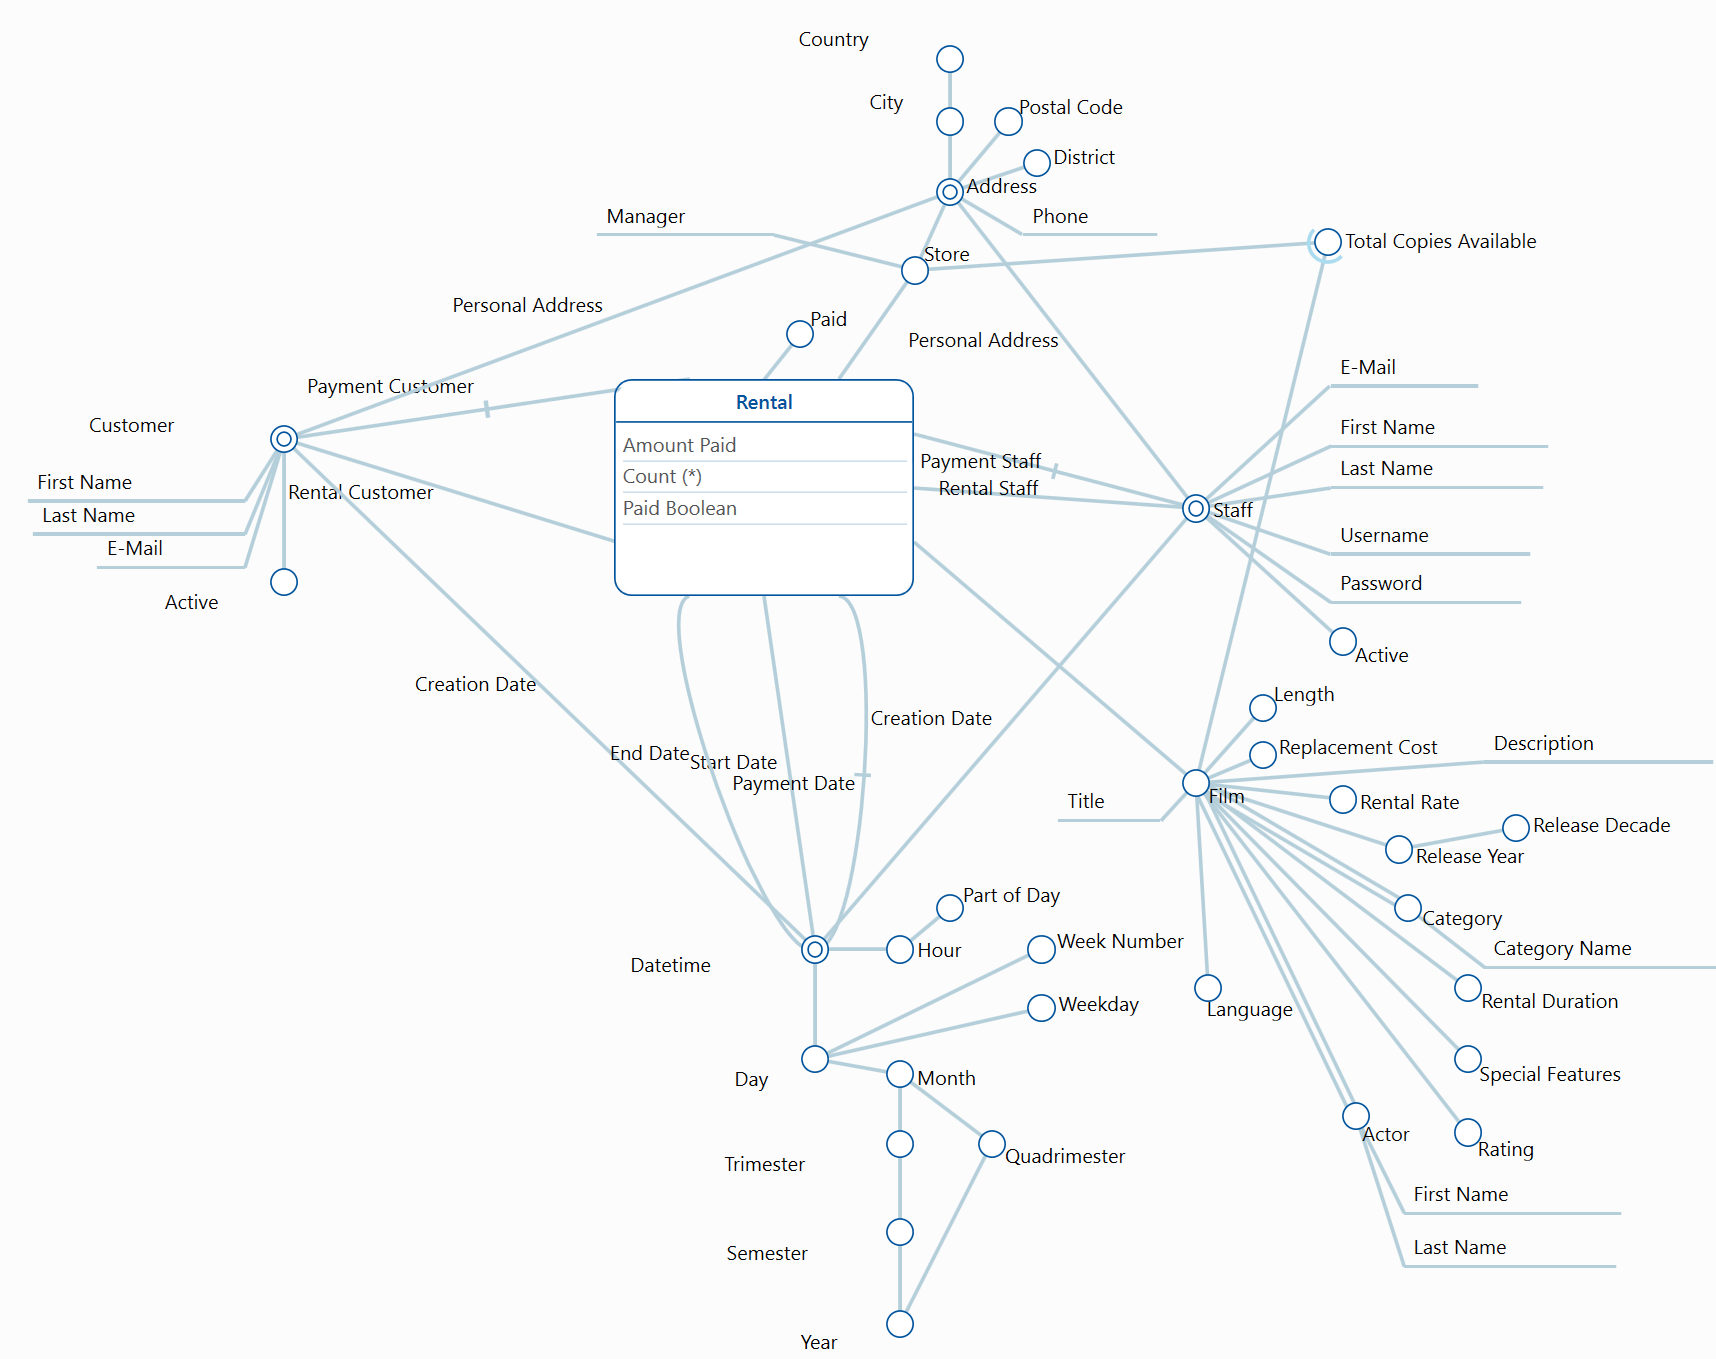
\includegraphics[width=1.2\textwidth, center, keepaspectratio=1]{{"../Dimensional Fact Model}.png}
\end{figure}
\vspace{-10mm}
\subsection{Observations}
The \textit{fact table} contains information about \textbf{Rentals} and \textbf{Payments}; from the original database schema, it is possible to see that the payment of a rental can be done at a different time than the rental itself. However, each payment refers to a single rental, so it is still possible to use a single fact table by making use of shared and optional dimensions, as explained below.

$\bullet$ \textbf{Measures:}
\vspace{-4mm}
\begin{itemize}
    \item \textbf{\textit{Amount paid:}} the measure contains how much a single rental was paid by a customer. As it is possible to have rentals for which the payment hasn't been done yet, it is suitable to have a specific value such as \textit{"Not paid"} to handle this situation.
    \item \textbf{\textit{Count (*):}} this measure is simply used to count the number of rentals that are done, regardless of the payment. It could be used, for instance, to discover which are the most popular movies in each store or country.
    \item \textbf{\textit{Paid\_bool:}} this boolean measure is used to distinguish between rentals for which a payment has been made or not. As an example, it can be used to measure the average payment rate for each store.
\end{itemize}
$\bullet$ \textbf{Dimensions:}
\vspace{-4mm}
\begin{itemize}
    \item \textbf{\textit{Paid\_dim:}} whether a rental is paid or not isn't only useful as a measure, but also as a dimension, to analyze only the rentals that were paid.
    \item \textbf{\textit{Customer:}} it was decided to include many different descriptive attributes (such as \textit{e-mail}) as the assignment requested to preserve all the information contained in the \textit{OLTP} database.\\
        The fact table is connected to the customer dimensions though 2 different arcs: one for the customer who made the rental, and one for the customer that made the payment. The second arc is optional, as some rentals might not have a payment associated to them. Moreover, by querying the existing database, it is possible to see that the customer who made the rental and the one who paid might be different.
    \item \textbf{\textit{Staff:}} this dimension is structured similarly to \textit{customer}. Once again, it is required to distinguish between the staff member related to the rental and the (optional) one related to the payment.
    \item \textbf{\textit{Store}}, \textbf{\textit{Customer}} and \textbf{\textit{Staff}} are all connected to the \textbf{\textit{Address}} dimension.
        It should be noted that the \textit{District} doesn't belong to the hierarchy of \textit{city} and \textit{country}, as there are cities that belong to multiple districts and viceversa. It could be assumed that a district belongs to a single country, but from the given description it isn't possible to say so.
        On the same line of thought, it could be possible to build a hierarchy from \textit{store} and \textit{manager}, if it was possible that a manager was in the lead of multiple stores. This can't however be determined from the information at disposal.
     \item \textbf{\textit{Date:}} the basic element of the hierarchy is \textit{datetime}, i.e. the full date with time and time-zone. From there, it is possible to infer the day, the month, etc.\\
         Similarly to \textit{Customer} and \textit{Staff} it is necessary to separate the dates of the rental and the one of the payment, which is optional. 
     \item \textbf{\textit{Film:}} this dimension is linked to multiple others attribute, such as \textit{Category}and \textit{Language}; moreover, it is possible to build a small hierarchy made of \textit{Release Year} and \textit{Release Decade}. The \textit{Special feature} attribute can be used to analyze whether having commentaries or trailers can impact the popularity of a movie. In practice, it would be better to convert the attribute to a set of binary columns, so that it is possible to separate the single features from each other. \\
         The \textbf{\textit{Total Copies Available}} dimension is used to keep track of how many copies of each movie are in the inventory of each store. This values aren't already in the \textit{OLTP} database, but can be easily computed from the \textit{inventory} table.
\end{itemize}

\end{document}
